

\documentclass[11pt, oneside]{article}   	% use "amsart" instead of "article" for AMSLaTeX format
\usepackage{geometry}                		% See geometry.pdf to learn the layout options. There are lots.
\geometry{letterpaper}                   		% ... or a4paper or a5paper or ... 
%\geometry{landscape}                		% Activate for rotated page geometry
\usepackage[parfill]{parskip}    		% Activate to begin paragraphs with an empty line rather than an indent
\usepackage{graphicx}				% Use pdf, png, jpg, or eps§ with pdflatex; use eps in DVI mode
								% TeX will automatically convert eps --> pdf in pdflatex		
\usepackage{amssymb}
\usepackage{amsmath} 
\usepackage{bm}
\usepackage{xcolor}
\usepackage{bbm}
\usepackage{bbold}
\usepackage[T1]{fontenc}
\usepackage{subfigure}
\usepackage[english]{babel}
\newtheorem{theorem}{Theorem}[subsection]
\newtheorem{corollary}{Corollary}[theorem]
\newtheorem{lemma}[theorem]{Lemma}
\newtheorem{mydef}{Definition}

%SetFonts

%SetFonts


\title{Clicking Data}
\author{}
\date{}							% Activate to display a given date or no date

\begin{document}
\maketitle
\section{General Notations}

\begin{itemize}
	
	\item {$c^j$: number of items clicked by user $j$}
	\item {$\mathcal{A}_j$: set of items clicked by user $j$, |$\mathcal{A}_j| = c_j$}
	\item {$\mathcal{A}_j^c$: set of items NOT clicked by user $j$, |$\mathcal{A}_j^c| = n-c_j$ }
	\item {$\bm{B}^j = \{b^j_1, ..., b^j_n\}$: a binary vector of length $n$, indicating user $j$'s clicks. $b^j_i$ = 1 if $i \in \mathcal{A}_j$, and 0 otherwise}
	
\end{itemize}
\section{Likelihood function for clicking data}
\section{Simulation results}
\subsection{Toy example set up}
In this section, we first simulate a dataset of $N = 20$ users, $n = 20$ items, $\bm{\rho}^0 = 1, ..., n$, and $\alpha^0 = 5$, by sampling from the Mallows distribution. The number of clicks for each user $c_j$ is drawn from a truncated poisson distribution, with a mean of 5 items, minimum of 1 item and maximum of 17 items. We recommend $ k = 2$ items for each user.  

\subsection{Comparison of $\bm{\rho}$}
A comparison of the distribution of $\bm{\rho}$ using the Mallows posterior and the pseudo-likelihood is shown on \textbf{Figure} \ref{fig:heat_rho}.
\begin{figure}[hbt!]
	\begin{minipage}[t]{.45\textwidth}
		\centering
		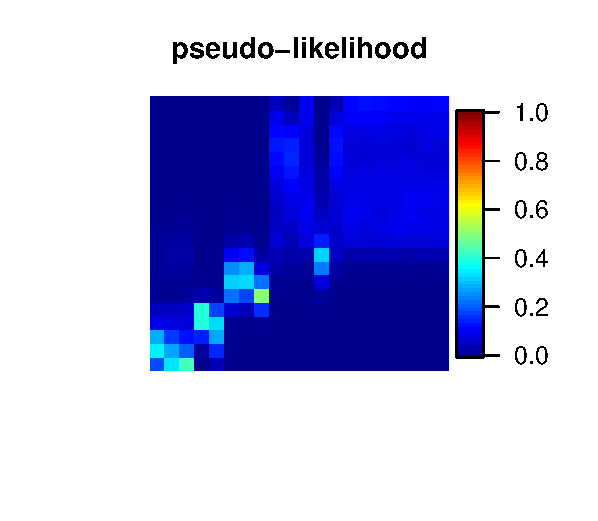
\includegraphics[width=\textwidth]{figures/clicking/Pseudo_rho_heat}
		
	\end{minipage}
	\hfill
	\begin{minipage}[t]{.45\textwidth}
		\centering
		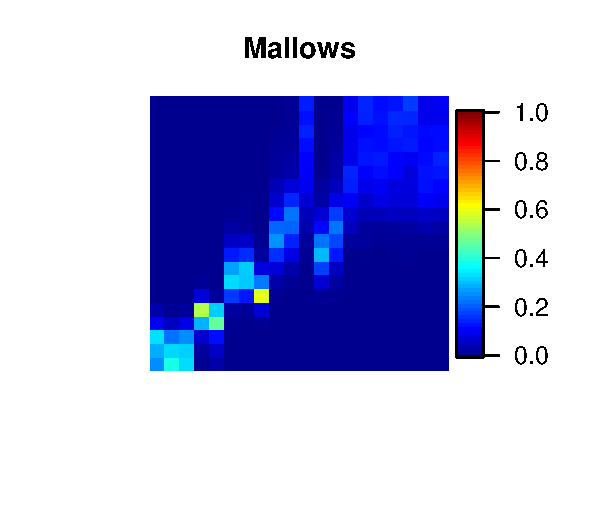
\includegraphics[width=\textwidth]{figures/clicking/Mallows_rho_heat}
		
	\end{minipage} 
	\caption{left: pseudo-likelihood, right: Mallows}
	\label{fig:heat_rho}
\end{figure}

\subsection{Heat plots of selected individual users}
Heat plots of 2 selected users are shown in \textbf{Figure} \ref{fig:heat_ind}. The distributions appear quite similar, except for a few items, in which using the pseudo-likelihood function produces a somewhat flatter distribution compared to using Mallows directly. 
\begin{figure}[hbt!]
	\begin{minipage}[t]{.45\textwidth}
		\centering
		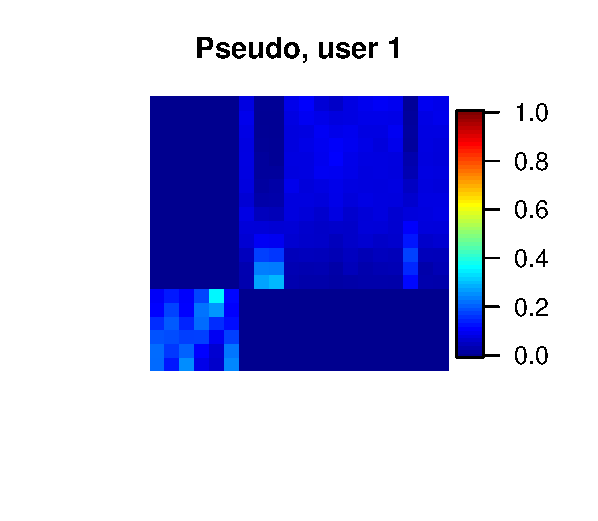
\includegraphics[width=\textwidth]{figures/clicking/pseudo_user1}
		
	\end{minipage}
	\hfill
	\begin{minipage}[t]{.45\textwidth}
		\centering
		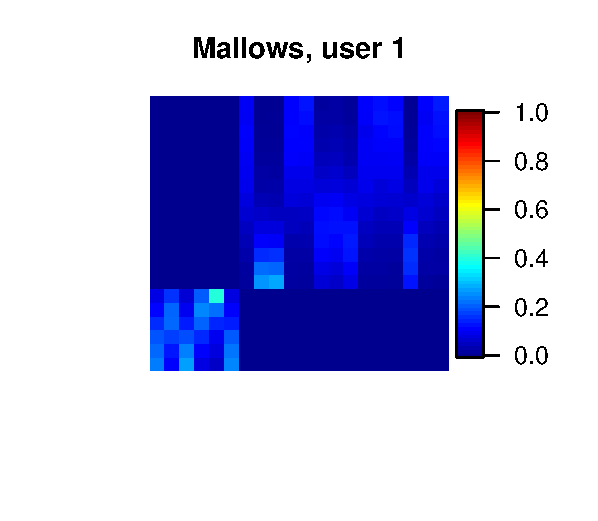
\includegraphics[width=\textwidth]{figures/clicking/mallows_user1}
		
	\end{minipage} 
	\begin{minipage}[t]{.45\textwidth}
	\centering
	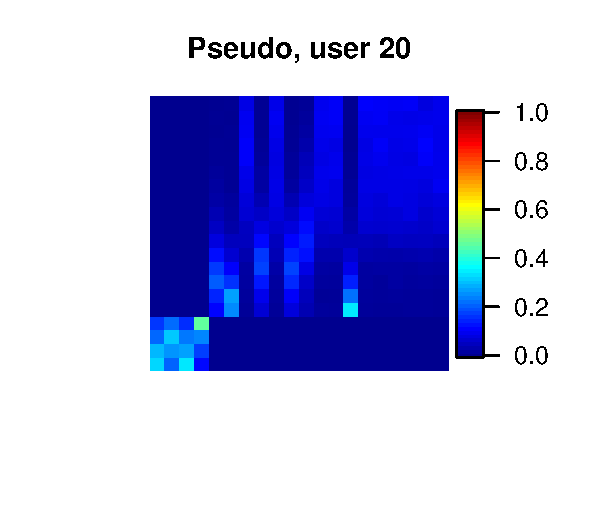
\includegraphics[width=\textwidth]{figures/clicking/pseudo_user20}
	
	\end{minipage}
	\hfill
	\begin{minipage}[t]{.45\textwidth}
		\centering
		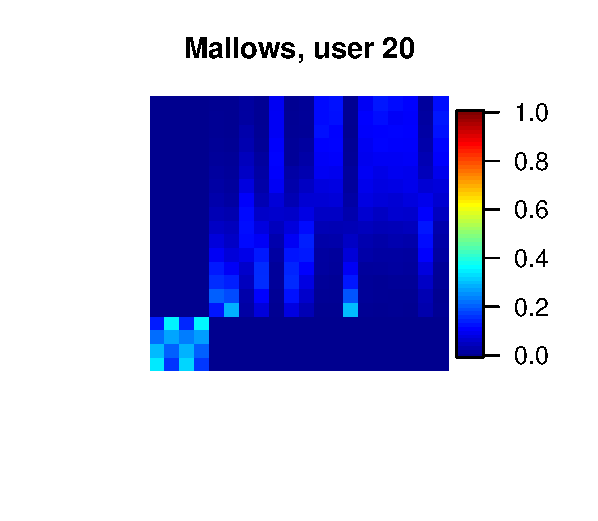
\includegraphics[width=\textwidth]{figures/clicking/mallows_user20}
		
	\end{minipage} 

	\caption{left: pseudo-likelihood, right: Mallows. The items are sorted according to the truth of the individual}
	\label{fig:heat_ind}
\end{figure}

\subsection{Recommendation accuracy}
In this particular toy example, the Pseudolikelihood 45\% of items are correctly recommended, while Mallows performs slightly better at 50\%.
\subsection{Special notes}
No Gaussian variation is introduced at this stage for the pseudo-likelihood; i.e., $\sigma = 0$. For each user $j$, the sequence for which items are to be sampled are based on a uniform distribution. (The V-ordering is tried out but don't seem to improve recommendation accuracy here). The $\alpha^0$ used for sampling is set at 10, instead of its real value 5. But the different choices of $\alpha^0$ don't seem to affect the resulted heat plots much.

\end{document}  